%Nachdem die theoretischen Grundlagen und der Aufbau des ALICE Experiment näher erläutert wurden, wird im folgenden die Vorgehensweise erklärt, wie $\pi^{0}$ gemessen werden.
%\newline
Die gewählten \textit{Cluster} nach den Kriterien aus Abschnitt \ref{s3s1s2} bestehen fast ausschließlich aus Photonen, und  Elektronen beziehungsweise Positronen aus der Konversion eines Photons.
\begin{figure}[tp]
\centering
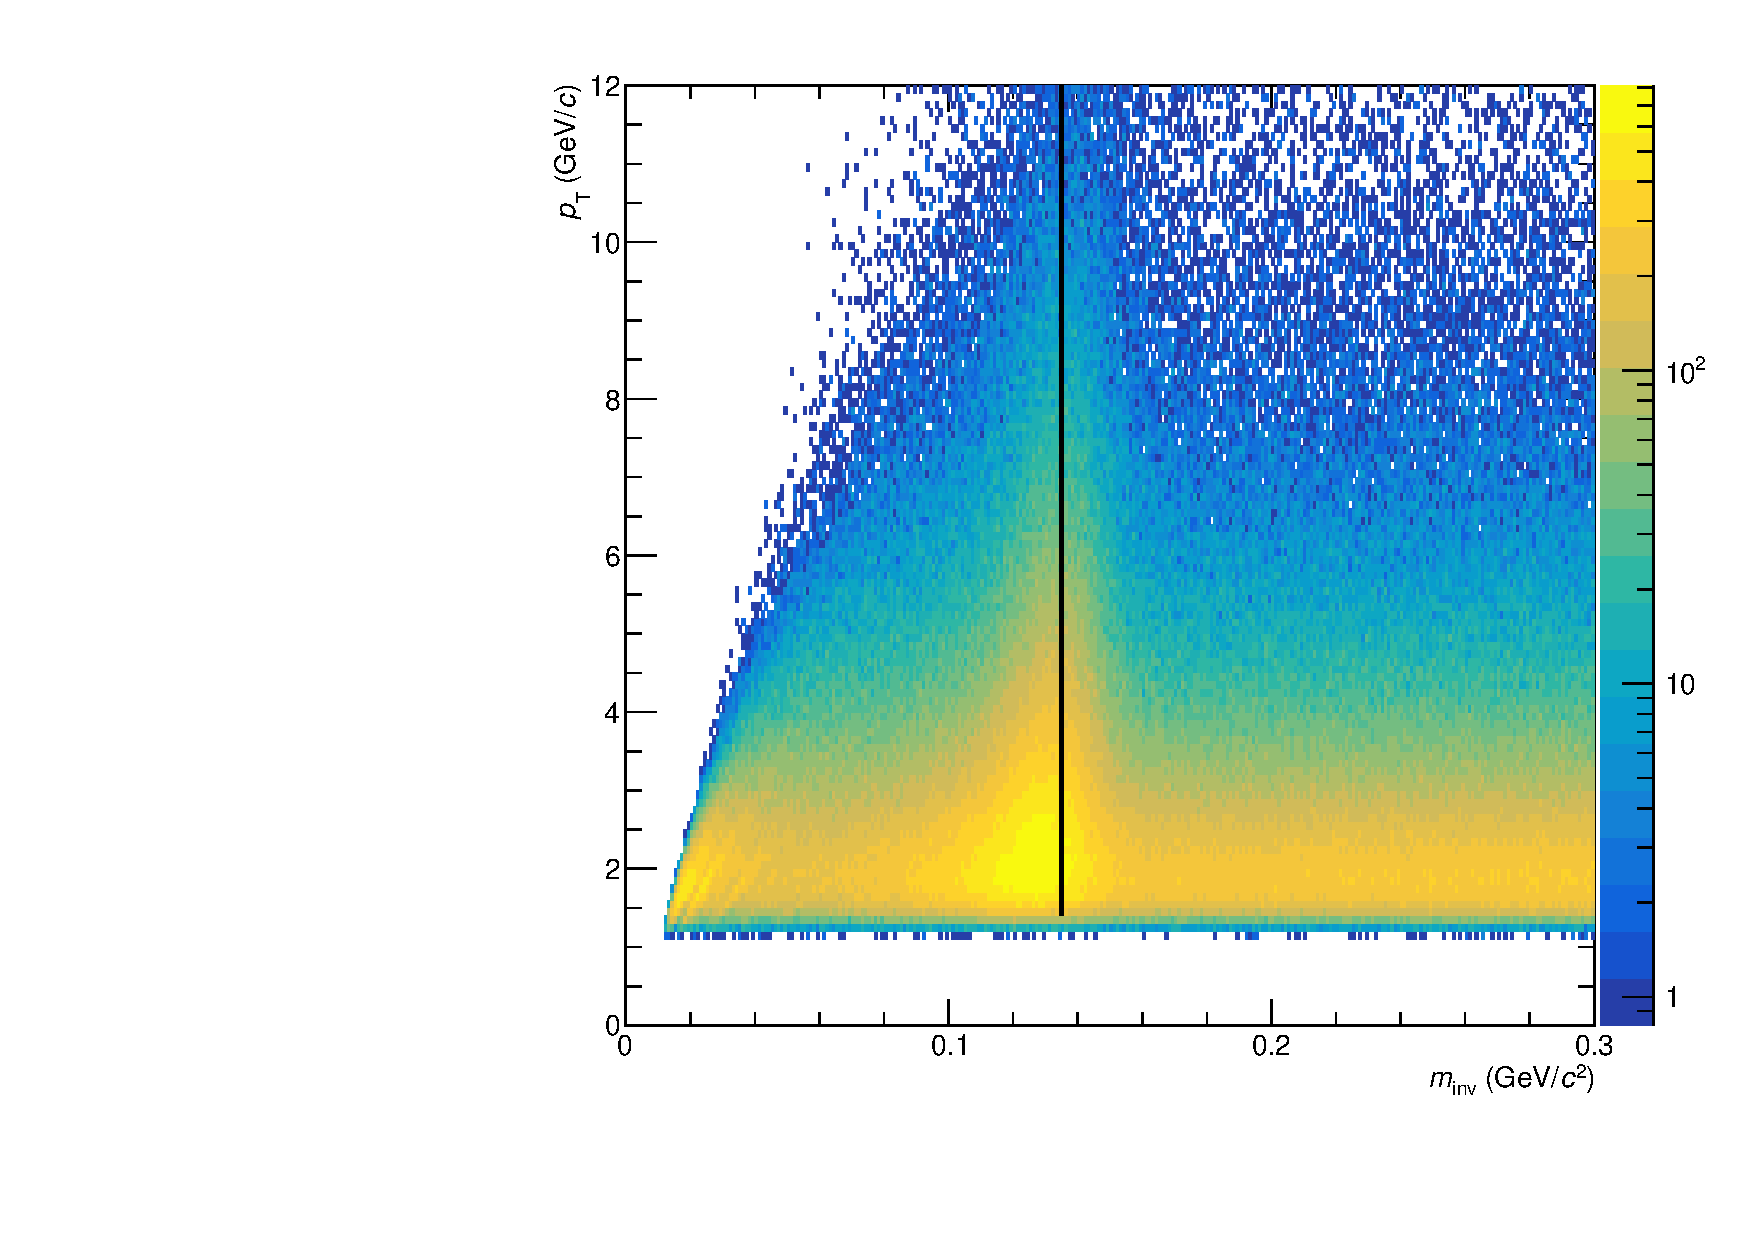
\includegraphics[width=.7\linewidth]{hInvMass_pT_Signal.pdf}
\caption{$p_\text{T}$ und $m_\text{inv}$ als Funktion der Anzahl von kombinierten  Cluster-Paaren aus der gleichen Kollision.
Die rote Linie liegt bei $m_{\text{inv}}\approx0\,135\text{ GeV/}c^{2}$, was in etwa der $\pi^{0}$ Masse entspricht, wo eine deutliche Häufung der Einträge sich abzeichnet.
Die schwarzen Linien stellen die Grenzen der $p_{\text{T}}$-Intervalle dar.}
\label{figInvMassPt_a}
\end{figure}
\newline
Um die Anzahl der detektierten $\pi^{0}$ zu messen, werden von Photonenkandidatenpaaren die invariante Masse und der Transversalimpuls nach Gleichungen \ref{eq_invmass} und \ref{eq_pt} bestimmt.
Da die Information fehlt, ob und welche Photonenkandidaten aus dem Zerfall eines $\pi^{0}$ stammen, werden alle Photonenkandidaten eines \textit{events} paarweise mit einander kombiniert.
Diese Methode wird als \textit{same event} Methode bezeichnet.
Abbildung \ref{figInvMassPt_a} zeigt die Anzahl der \textit{Clusterpaare} in Abhängigkeit der invarianten Masse $m_{\text{inv}}$ und des Transversalimpulses $p_{\text{T}}$.
Durch die paarweise Kombination aller Photonenkandidaten eines \textit{Events} gibt es sowohl Kombinationen von Photonenkandidaten, die aus dem Zerfall eines $\pi^{0}$ stammen, als auch Photonenkandidaten, die nicht über den Zerfall eines einzelnen $\pi^{0}$ zusammenhängen.
\newline
Die Summe aller \textit{Clusterpaare}, die aus einem Zerfall eines $\pi^{0}$ kommen, wird als Signal bezeichnet.
Es zeichnet sich eine Häufung der Datenpunkte um $m_{\text{inv}}\approx 0\,135\text{ GeV}/c^{2}$, also um die Masse des $\pi^{0}$, ab.
Dieser Häufung liegt vor allem das Signal zugrunde.
Da Photonen durch Paarbildung in ein Elektron und ein Positron konvertieren können, bestehen einige Photonenkandidaten aus \textit{Clustern} aus nur einem der beiden Konversionsprodukte.
Diese Photonenkandidaten besitzen eine geringere Energie, als das eigentliche Photon besaß.
Durch Kombinationen mit diesen Photonenkandidaten entstehen Einträge bei einer invarianten Masse, die meistens geringer ist als die Masse von $\pi^{0}$, wenn beide Photonenkandidaten dem selben $\pi^{0}$ entstammen.
Deshalb wird bei invarianten Massen $m_\text{inv}<0\,135\text{ GeV}/c^{2}$ ein Teil des Signals erwartet.
\newline
Alle \textit{Clusterpaare}, die nicht zum Signal zählen, bilden den Untergrund, der in zwei Teile unterteilt wird, dem kombinatorischen oder auch unkorrelierten Untergrund und dem korrelierten Untergrund.
Dem korrelierten Untergrund liegen paarweise Kombinationen von Photonenkandidaten zugrunde, zwischen denen eine Korrelation besteht.
Das heißt, dass die Photonenkandidatenpaare nicht aus dem Zerfall eines einzelnen $\pi^{0}$ stammen, aber über andere Zerfälle zusammenhängen.
Durch die paarweise Kombination unkorrelierter Photonenkandidaten entsteht der unkorrelierte Untergrund.
\newline
Aufgrund der Anforderung an den Öffnungswinkel werden stetig mehr Kombinationsmöglichkeiten von Photonenkandidaten ausgeschlossen.
Die ausgeschlossenen Kombinationen liegen im Bereich kleiner invarianter Massen weshalb es bei bei kleinem $m_{\text{inv}}$ keine Datenpunkte gibt.
Das führt dazu, dass mit steigendem $p_{\text{T}}$ immer mehr Signal nicht rekonstruierbar wird.
\newline
Die Anzahl der $\pi^{0}$ weist eine $p_{\text{T}}$-Abhängigkeit auf.
Deshalb wird die Verteilung aus Abbildung \ref{figInvMassPt_a} in einzelnen $p_{\text{T}}$-Intervallen analysiert.
Die Intervalle werden so gewählt, dass sie möglichst klein sind, während die statistischen Unsicherheiten der Datenpunkte nicht zu groß werden.
\begin{figure}[tbp]
\centering
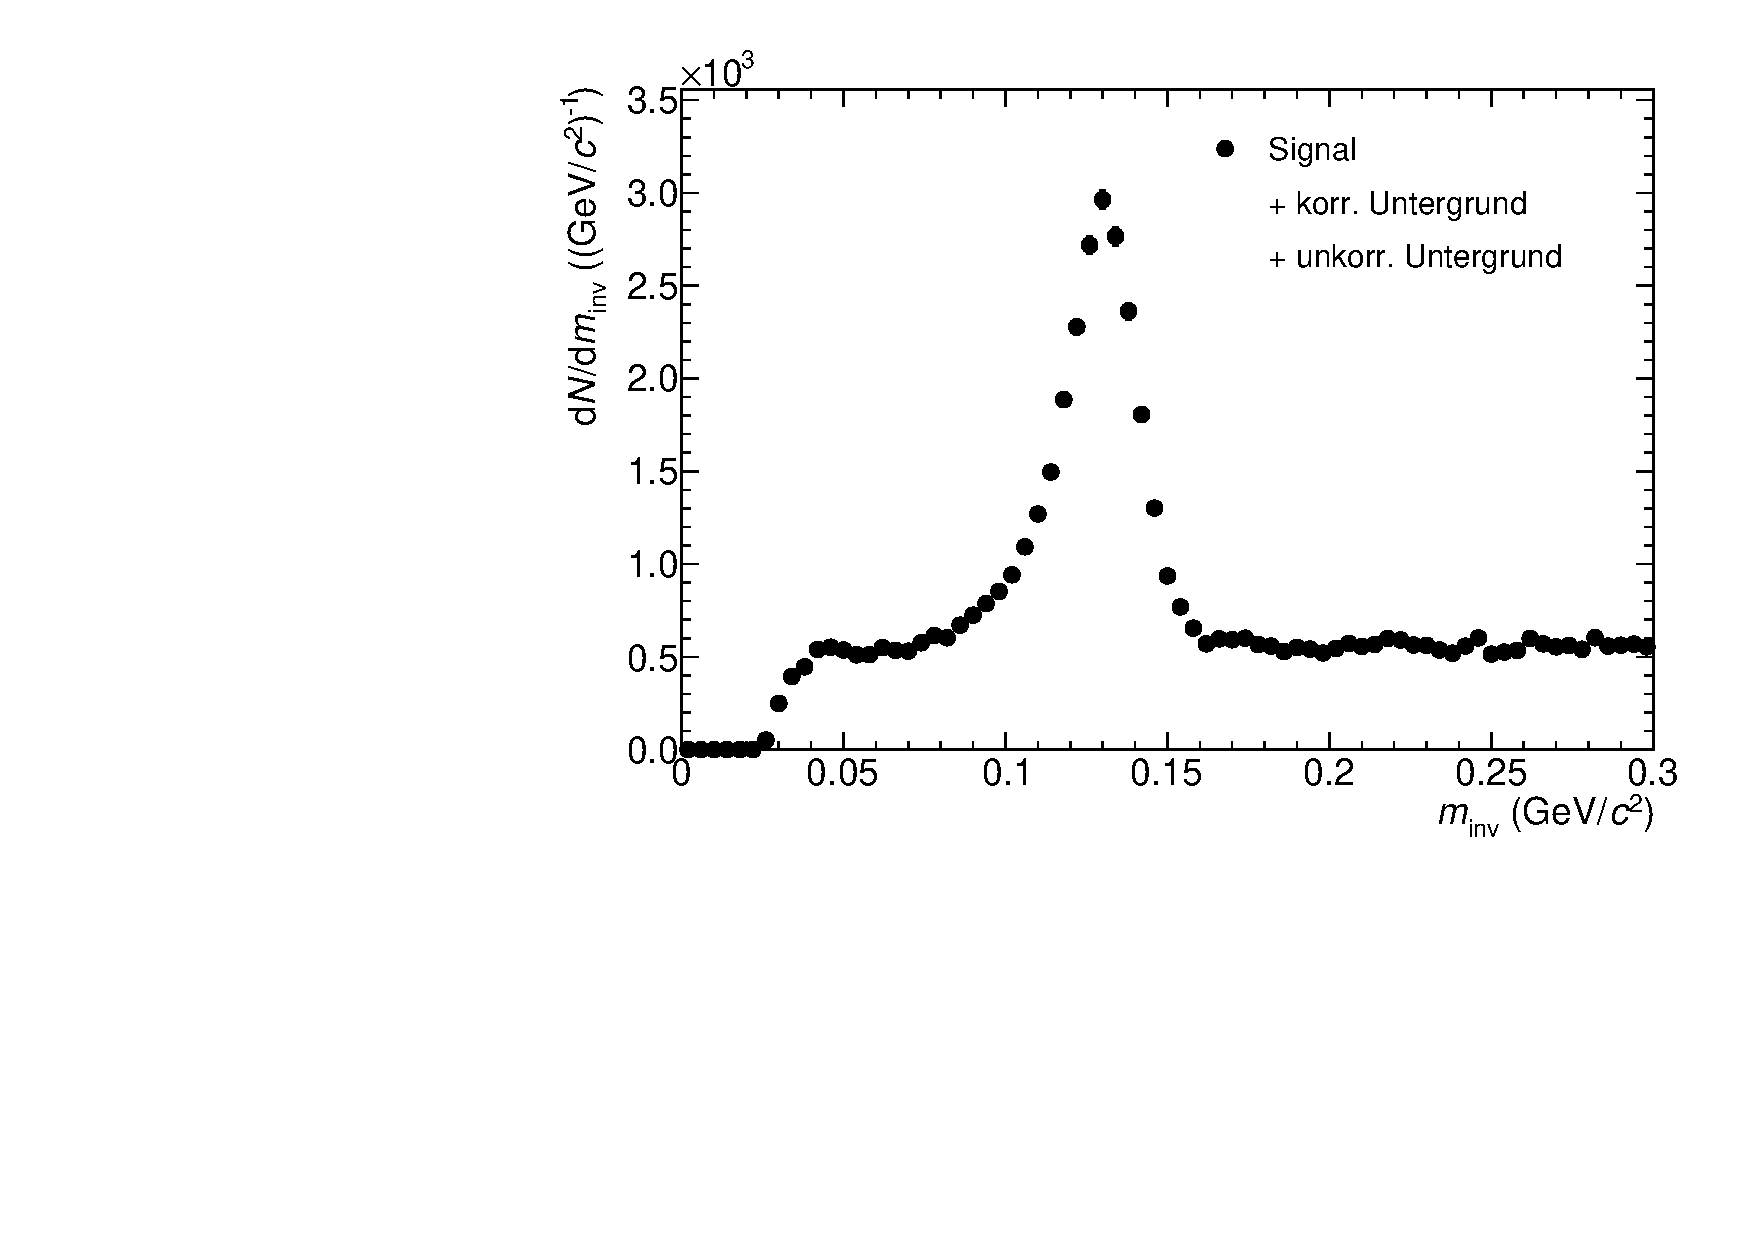
\includegraphics[width=.75\linewidth]{hSignalPlusBkg.pdf}
\caption{Projektion von Abbildung \ref{figInvMassPt_a} im $p_{\text{T}}$-Intervall $(3,2 - 3,4) (\text{GeV/}c)$. Es ist ein deutlicher Peak um $m_{\pi^{0}} \approx 0\,135\text{ GeV/}c^{2}$ zu erkennen, aber auch Untergrund, da das Signal zu höheren Massen gaußförmig abklingen sollte. Bei $m_{\text{inv}} < m_{\pi^{0}}$ kann Signal vorliegen, das aus konvertierten Photonen besteht, weshalb eine Aussage über die Form, beziehungsweise den Untergrund dort schwer möglich ist.}
\label{figSignalPlusBkg}
\end{figure}
\newline
Abbildung \ref{figSignalPlusBkg} zeigt die Anzahl der \textit{Clusterpaare} in Abhängigkeit der invariante Massen im $p_{\text{T}}$-Intervall von $(3\,2 - 3\,4)(\text{GeV}/c)$.
Die in Abbildung \ref{figInvMassPt_a} beschriebene Anhäufung der Datenpunkten zeigt sich auch hier deutlich und wird im Folgenden als Peak bezeichnet.
Der Peak besteht wie zuvor erwähnt hauptsächlich aus Signal.
\newline
Im folgenden Abschnitt wird eine Methode zur Abschätzung des unkorrelierten Untergrunds vorgestellt. 